\documentclass[a4paper,kul]{kulakarticle} %options: kul or kulak (default)

\usepackage[utf8]{inputenc}
\usepackage[english]{babel}
\usepackage{graphicx}
\usepackage{subcaption}
\newlength{\twosubht}
\newsavebox{\twosubbox}
\graphicspath{{../Figures/}{../Matlab/}{/}}
\usepackage[outdir=./]{epstopdf}

\usepackage{tikz}
\usetikzlibrary{shapes,arrows}

\usepackage{amsmath}
\usepackage{amsthm}
\usepackage{amssymb}
\usepackage{gensymb}
\setcounter{MaxMatrixCols}{21}

\usepackage{etoolbox,refcount}
\usepackage{multicol}

\newcounter{countitems}
\newcounter{nextitemizecount}
\newcommand{\setupcountitems}{%
	\stepcounter{nextitemizecount}%
	\setcounter{countitems}{0}%
	\preto\item{\stepcounter{countitems}}%
}
\makeatletter
\newcommand{\computecountitems}{%
	\edef\@currentlabel{\number\c@countitems}%
	\label{countitems@\number\numexpr\value{nextitemizecount}-1\relax}%
}
\newcommand{\nextitemizecount}{%
	\getrefnumber{countitems@\number\c@nextitemizecount}%
}
\newcommand{\previtemizecount}{%
	\getrefnumber{countitems@\number\numexpr\value{nextitemizecount}-1\relax}%
}
\makeatother    
\newenvironment{AutoMultiColItemize}{%
	\ifnumcomp{\nextitemizecount}{>}{3}{\begin{multicols}{2}}{}%
		\setupcountitems\begin{itemize}}%
		{\end{itemize}%
		\unskip\computecountitems\ifnumcomp{\previtemizecount}{>}{3}{\end{multicols}}{}}

\usepackage{pdflscape}

\date{Academic year 2021 -- 2022}
\address{
  Faculty of Engineering Science \\
  Department of Mechanical Engineering \\
  Control theory \texttt{[H04X3a]}}
\title{Report Assignment 3: State Feedback and State Estimation}
\author{Matthias Derez, Toon Servaes}


\begin{document}

\maketitle

\tableofcontents
\listoffigures
\listoftables

\tikzstyle{block} = [draw, rectangle, 
minimum height=3em, minimum width=6em]
\tikzstyle{blocksmall} = [draw, rectangle, 
minimum height=3em, minimum width=3em]
\tikzstyle{sum} = [draw, circle, node distance=1cm]
\tikzstyle{input} = [coordinate]
\tikzstyle{output} = [coordinate]
\tikzstyle{pinstyle} = [pin edge={to-,thin,black}]



\newpage
\section{Design of the State Feedback Controller}
In this Section, a state feedback controller is designed in order to control the position of the cart while driving on a straight line. This position control loop is then added on top of the velocity controllers designed in Assignment 2. 

\subsubsection*{Input \& Output}
Figure \ref{fig:flowdiagram} visualizes the discrete time LTI system that is examined in this assignment. The input and output are given by:
\begin{equation}
	\begin{split}
	\text{input } u(t) &= v(t) = R\omega(t) = \dot{x}(t) \\
	\text{output } y(t) &= -x(t)
	\end{split}
\end{equation}
where $v(t)$ is the velocity of the cart, $R$ the radius of the wheels and $\omega$ the rotational velocity of the wheels. The minus sign in the output equation is due to choice of the coordinate system, so that $-x$ represents a positive value. 

\subsubsection*{State Space Model}
There is only one state, the position $x$, so the matrices in the state equation (and measurement equation) are scalars. 
\\\\
Continuous state space model:
\begin{equation}
\left\{
	\begin{split}
	\dot{x}(t) &= v(t) = u(t) \qquad &\text{state equation} \\
	y(t) &= -x(t) &\text{measurement equation}
	\end{split}
	\right.
\end{equation}
Discretization using Forward-Euler scheme:
\begin{equation}
	\dot{x}[k] = \frac{x[k+1] - x[k]}{T_s} + O(T_s^2)
\end{equation}
leads to:
\begin{equation}
\left\{
\begin{split}
\dot{x}[t+1] &= x[k] + T_s u[k] \qquad &\text{state equation} \\
y[t] &= -x[t] &\text{measurement equation}
\end{split}
\right.
\end{equation}
with $T_s$ the sampling time of $0.01$ s. From the general discretized state space form, one can deduce that $A = 1$, $B = T_s$, $C = -1$ and $D = 0$.

\subsubsection*{Close Loop Transfer Function}
Assuming full state feedback, the closed loop transfer function is:
\begin{equation}
	\begin{split}
	H(z) = \frac{Y(z)}{R(z)} &= (C-DK)(z - A + BK)^{-1}B + D \\
	&= -(z-1 + T_s K)^{-1} T_s \\
	&= \frac{-T_s}{z-1+T_sK}
	\end{split}
\end{equation}
with $K$ the state feedback gain. Subsequently, the closed loop system has one pole, which is located at
\begin{equation}
	p_d = 1 - T_s K
\end{equation}
This equation indicates that the pole moves to the left for increasing K, or inversely, move to the right for decreasing K, as seen in Figure \ref{fig:poles}. In the discrete time domain, the system is stable if the poles are within the unit circle. For this particular system, this means $0 < K < 200$ Hz.


\begin{figure}[htp]
	\centering
	\resizebox{.7\linewidth}{!}{
	\begin{tikzpicture}[auto, node distance=2cm,>=latex']
	% We start by placing the blocks
	\node [input, name=input] {};
	\node [sum, right of=input, node distance = 1.8cm] (sum) {};
	\node [block, right of=sum, node distance=3cm] (controller) {$qx = Ax + Bu$};
	\draw [->] (sum) -- node[name=extra, anchor=north] {$u[k]$} (controller);
	\node [blocksmall, right of=controller,
	node distance=3.5cm] (system) {$C$};
	% We draw an edge between the controller and system block to 
	% calculate the coordinate u. We need it to place the measurement block. 
	\draw [->] (controller) -- node[name=u] {$x[k]$} (system);
	\node [sum, right of=system, node distance=2cm] (disturbance) {};
	\node [blocksmall, above of=u, node distance = 1.3cm] (gd) {$D$};
	\node [output, right of=disturbance] (output) {};
	\node [blocksmall, below of=controller, node distance = 1.5cm] (measurements) {$-K$};
	
	% Once the nodes are placed, connecting them is easy. 
	\draw [draw,->] (input) -- node {$r[k]$} (sum);
	\draw [->] (system) -- node[pos=0.97] {$+$} (disturbance);
	\draw [->] (disturbance) -- node [name=y] {$y[k]$}(output);
	\draw [->] (extra) |- node {} (gd);
	\draw [->] (gd) -| node {} (disturbance);
	\draw [->] (u) |- (measurements);
	\draw [->] (measurements) -| node[pos=0.99] {$+$}  (sum);
	\end{tikzpicture}}
	\caption{Flow diagram of the closed loop system. \cite{tikz}}
	\label{fig:flowdiagram}
\end{figure}
\newpage
\noindent Furthermore, a pole that is close to the unit circle, e.g. for $K = 10$ or $K = 190$, leads to a slower responding system. Equivalently, a pole that is closer to the origin leads to a faster response. These conclusions are demonstrated by Figure \ref{fig:impulse_response}. The limit cases are when, on the one hand, the pole is located on the unit circle itself, meaning that the system is on the edge of stability. On the other hand, a pole which lies at the origin corresponds to an infinitely fast system, i.e. a pure time delay. This would however mean that the control signal will be infinitely large, thus saturating the actuators. So there is a trade-off between response time and cost in terms of required actuation signal. Both of these limit cases are depicted in Figure \ref{fig:impulse_response}.




\begin{figure}[htp!]
	\centering
	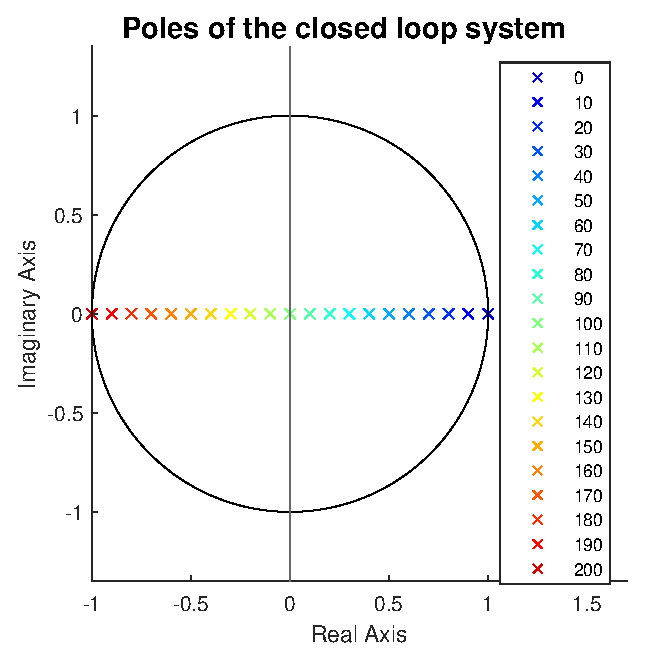
\includegraphics[width=0.5\linewidth]{poles.eps}
	\caption{Pole locations of the closed-loop system for varying values of the state feedback gain.}
	\label{fig:poles}
\end{figure}


\begin{figure*}[htp!]
	\centering
	\begin{subfigure}[b]{0.48\textwidth}
		\centering
		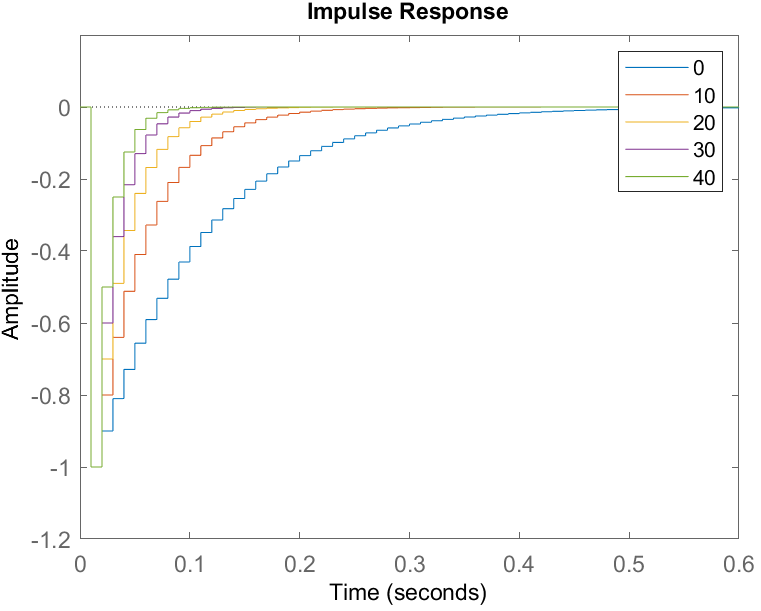
\includegraphics[width=\textwidth]{impulse_response1_cropped.pdf}
	\end{subfigure}
	\hfill
	\begin{subfigure}[b]{0.48\textwidth}  
		\centering 
		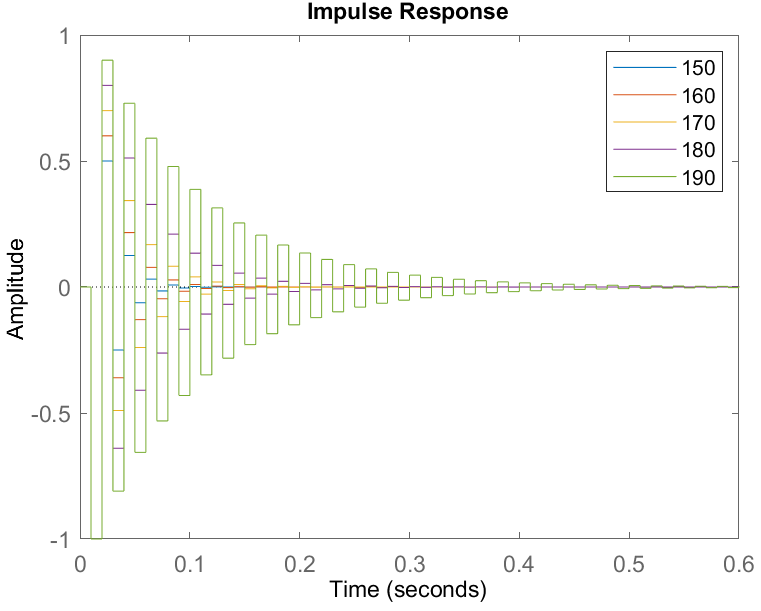
\includegraphics[width=\textwidth]{impulse_response2_cropped.pdf}
	\end{subfigure}
	
	\begin{subfigure}[b]{0.48\textwidth}  
		\centering 
		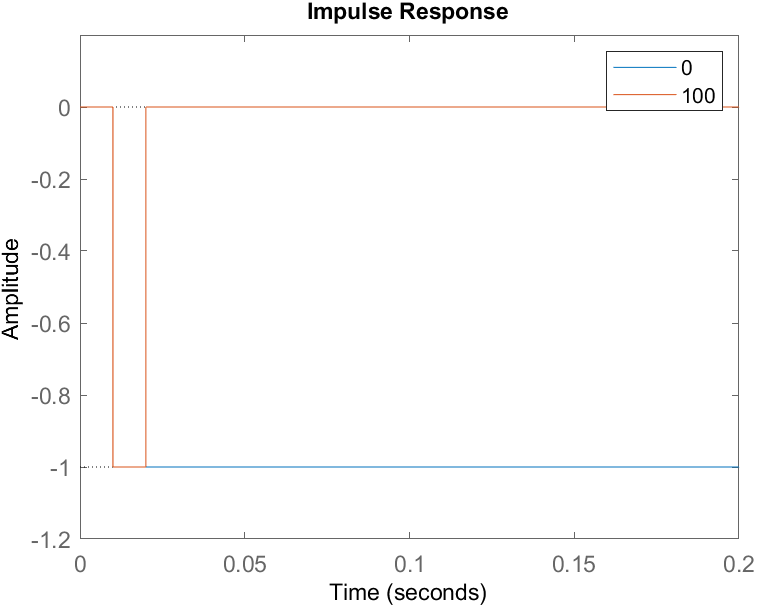
\includegraphics[width=\textwidth]{impulse_response3_cropped.pdf}
	\end{subfigure}
	\caption{Impulse response of the closed-loop system for varying values of the state feedback gain K.} 
	\label{fig:impulse_response}
\end{figure*}

\newpage
\section{Kalman Filter}
As previously elaborated, the measurement equation is equal to 
\begin{equation}
	y[t] = -x[t]
	\label{eq:eq7}
\end{equation}
so the C and D matrices of the state-space model are scalar values, respectively $-1$ and $0$. In this Section, these values are used to validate the principles of the Kalman filter on this system. To this extent, some mathematical derivations are done. 

\subsubsection*{Kalman gain}

Firstly, an expression for the time-varying Kalmain gain $L_{k+1}$ is derived as a function of the state estimate covariance $\hat{P}_{k|k}$, the process noise covariance $Q$ and measurement noise covariance $R$. This starts from the following equations in Chapter 10 of \textit{Control Theory - Handouts} \cite{slidescontroltheory}:

\begin{align}
	\mathbf{L}_{k+1} &= \mathbf{\hat{P}}_{k+1|k} \mathbf{C}^T S_{k+1}^{-1} \label{eq:eq8}\\
	S_{k+1} &= \mathbf{C \hat{P}}_{k+1|k} \mathbf{C}^T + R_{k+1} \label{eq:eq9}\\
	\mathbf{\hat{P}}_{k+1|k} &= \mathbf{A} \mathbf{\hat{P}}_{k|k} \mathbf{A}^T + \mathbf{Q}_k \label{eq:eq10}
\end{align}

\noindent All matrices and vectors are scalar values in this specific system, so from now on, the boldface notation is left out. Inserting Equations (\ref{eq:eq8}) and (\ref{eq:eq9}) in Equation (\ref{eq:eq10}) and using $A = 1$ and $C = -1$ yields:
\begin{equation}
	\begin{split}
	L_{k+1} &= -\left( \hat{P}_{k|k} + Q_k \right) \left( \hat{P}_{k+1|k} + R_{k+1} \right)^{-1} \\
	&= - \frac{\hat{P}_{k|k} + Q_k}{\hat{P}_{k+1|k} + R_{k+1}} \\
	&= - \frac{\hat{P}_{k|k} + Q_k}{\hat{P}_{k|k} + Q_k + R_{k+1}}
	\end{split}
	\label{eq:eq11}
\end{equation}
where Equation (\ref{eq:eq10}) was used again in the last step.
\\\\
Taking the limit for $Q_k \rightarrow \infty$ results in $L_{k+1} = -1$, which in turn leads to $\hat{x}_{k+1|k+1} = -y_{k+1}$. This is literally the measurement equation of the state-space model (\ref{eq:eq7}). One can explain this as follows: the larger $Q$, the greater the variation of the process noise, the less confidence in the model. Or equivalently, the more confidence in the measurement. In the extreme case, i.e. $Q_k \rightarrow \infty$, one has so little confidence in the model that the state equation is entirely neglected. 
\\\\
Next, taking the limit for $R_{k+1} \rightarrow \infty$ prompts $L_{k+1} = 0$, which results in $\hat{x}_{k+1|k+1} = \hat{x}_{k+1|k}$. The a priori state estimate is equal to the a posteriori state estimate, meaning that the correction step in the Kalman filter process is neglected. This is yet again easily explainable: the larger $R$, the greater the variation of the measurement noise, the less confidence in the measurement. Or equivalently, the more confidence in the model. The extreme case $R_{k+1} \rightarrow \infty$ has so little confidence in the measurement that the innovation residual is completely not taken into account, thus eliminating the correction step.

\subsubsection*{Next state estimate covariance}
Secondly, an expression for the next state estimate covariance $\hat{P}_{k+1|k+1}$ is derived as a function of the previous state estimate covariance $\hat{P}_{k|k}$, the process noise covariance $Q$ and measurement noise covariance $R$. Again, starting from an equation given in the handouts: 
\begin{equation}
	\hat{P}_{k+1|k+1} = (1 - L_{k+1} C)\hat{P}_{k+1|k} = (1 + L_{k+1})\hat{P}_{k+1|k}
\end{equation}
Using Equations (\ref{eq:eq10}) and (\ref{eq:eq11}) yields:
\begin{equation}
	\begin{split}
	\hat{P}_{k+1|k+1} &= \left(1 - \frac{\hat{P}_{k|k} + Q_k}{\hat{P}_{k|k} + Q_k + R_{k+1}}\right) \hat{P}_{k+1|k} \\
	&= \frac{R_{k+1}}{\hat{P}_{k|k} + Q_k + R_{k+1}}\left(\hat{P}_{k|k} + Q_k\right)
	\end{split}
	\label{eq:eq13}
\end{equation}

\noindent Taking the limit for $Q_k \rightarrow \infty$ results in $\hat{P}_{k+1|k+1} = R_{k+1}$. Again,  $Q_k \rightarrow \infty$ indicates that there is zero confidence in the model, so only the measurements get used to adapt the state estimate. This way, the reliability of the estimator is purely based on the reliability of the measurement. In other words, the uncertainty on the state estimate evolves according to the measurement noise covariance. Whereas this uncertainty evolves depending on both the model and the measurements in normal operation of the filter.
\\\\
Further, the limit for $R_{k+1} \rightarrow \infty$ prompts $\hat{P}_{k+1|k+1} = \hat{P}_{k|k} + Q_k = \hat{P}_{k+1|k}$. Once more, $R_{k+1} \rightarrow \infty$ indicates zero confidence in the measurements. The a priori covariance matrix of the estimation error is equal to the a posteriori covariance matrix, so the correction step in neglected. In other words, the reliability of the estimator is purely based on the reliability of the model. In normal operation of the filter, $\hat{P}_{k+1|k+1} \preceq \hat{P}_{k+1|k}$, meaning that the uncertainty of the state estimate decreases, whereas in this limit case, the uncertainty does not decrease after the correction step, but it stays the same.

\subsubsection*{Steady state covariance}
Now, an expression for the steady state covariance $\hat{P}_\infty$ and the related Kalman gain $L_\infty$ is obtained as a function of $Q$ and $R$. For this, $\hat{P}_{k|k} = \hat{P}_{k+1|k+1} = \hat{P}_\infty$, $R_{k+1} = R_{\infty}$ and $Q_k = Q_\infty$ are inserted in Equation (\ref{eq:eq13}):
\begin{equation}
	\hat{P}_\infty = \frac{R_{\infty}}{\hat{P}_{\infty} + Q_\infty + R_{\infty}}\left(\hat{P}_{\infty} + Q_\infty\right)
\end{equation}
Solving for $\hat{P}_\infty$ gives:
\begin{equation}
	\hat{P}_\infty = \frac{-Q_\infty \pm \sqrt{Q_\infty^2 + 4R_\infty Q_\infty}}{2}
\end{equation}
As all covariances must be positive numbers, the only solution for the steady state covariance is: 
\begin{equation}
\hat{P}_\infty = \frac{-Q_\infty + \sqrt{Q_\infty^2 + 4R_\infty Q_\infty}}{2}
\label{eq:eq16}
\end{equation}
Analogously, these steady state covariances are inserted in Equation (\ref{eq:eq11}) in order to find the related steady state Kalman gain:
\begin{equation}
L_\infty = - \frac{\hat{P}_\infty + Q_\infty}{\hat{P}_\infty + Q_\infty + R_\infty}
\label{eq:eq17}
\end{equation}
With $\hat{P}_\infty$ equal to Equation (\ref{eq:eq16}), $L_\infty$ is likewise expressed as a function of the steady state process noise covariance $Q_\infty$ and the steady state measurement noise covariance $R_\infty$.
\\\\
In steady state, i.e. $k \rightarrow \infty$, the optimal Kalman gain $L_{k+1}$ should converge to the estimator gain $L$ of a Linear Quadratic Estimator. This is verified by computing $L_\infty$ for various numerical values of $Q_\infty$ and $R_\infty$ using the derived equation. It is then compared to the result using the \texttt{dlqr(A',A'*C',Q,R)'} command in \texttt{Matlab}. E.g. $Q = 0.01$ and $R = 0.01$ leads to $L = -0.9161$ in both cases. One can conclude that the derived formula is correct.

\subsubsection*{Closed loop pole of the LQE}
Lastly, an expression for the closed-loop pole of the Linear Quadratic Estimator is derived as a function of $\frac{Q}{R}$. Generally, the estimator state equation is given by 
\begin{equation}
	\hat{x}_{k+1} = (A-LC) \hat{x}_k + (B-LD) u_k + L y_k
\end{equation}
In this way, the closed loop poles of the estimator are calculated as the eigenvalues of the matrix (A-LC):
\begin{equation}
	\text{det}(p_d I - (A-L_\infty C)) = 0
\end{equation}
Using the previously calculated scalar values of $A$ and $C$ and using Equations (\ref{eq:eq16}) and (\ref{eq:eq17}) yields:
\begin{equation}
	\begin{split}
		p_d &= 1 + L_\infty \\
		&= 1 - \frac{\hat{P}_\infty + Q_\infty}{\hat{P}_\infty + Q_\infty + R_\infty} \\
		&= \frac{R_\infty}{\hat{P}_\infty + Q_\infty + R_\infty} \\
		&= \frac{2R_\infty}{-Q_\infty + \sqrt{Q_\infty^2 + 4R_\infty Q_\infty} + 2Q_\infty + 2R_\infty} \\
		&= \cfrac{2}{\cfrac{Q_\infty}{R_\infty} + 2 + \sqrt{\left(\cfrac{Q_\infty}{R_\infty}\right)^2 + \cfrac{4Q_\infty}{R_\infty}}}
	\end{split}
\end{equation}

\noindent From this equation, one can deduce that the pole goes to zero with increasing $\frac{Q}{R}$. Inversely, for decreasing ratio ($\frac{Q}{R} \rightarrow 0$), the value of the pole shifts towards $1$. These conclusions are verified by Figure \ref{fig:poles_LQE}. For $\frac{Q}{R} = 0$, the pole lies on the unit circle, which implies that the system is unstable for this ratio. This is the only $\frac{Q}{R}$ - value that leads to instability, because, as depicted by the figure, the poles move towards the centre of the unit circle for increasing values of the ratio. In turn, it means that the systems responds faster and faster. This can easily be explained: the larger $\frac{Q}{R}$, the more confidence in the measurement. Subsequently, the system is more sensitive to measurement noise, which complies with a faster responding system.

\begin{figure}[htp!]
	\centering
	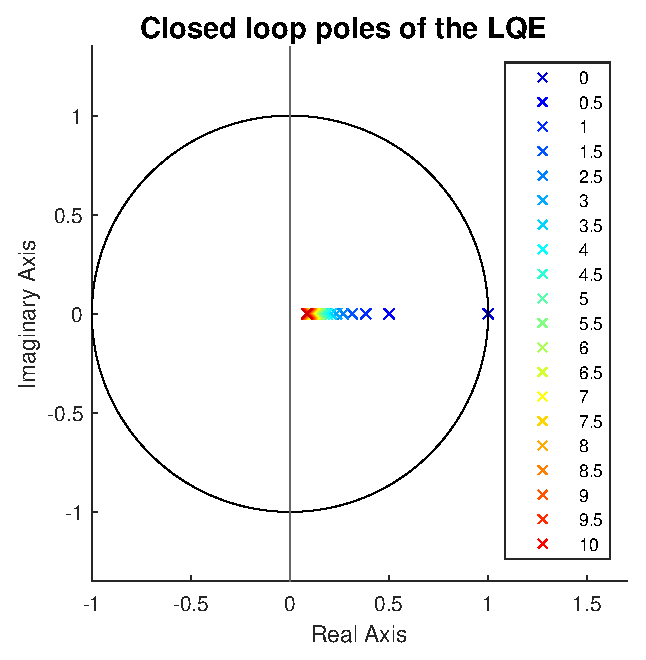
\includegraphics[width=0.5\linewidth]{poles_LQE.eps}
	\caption{Closed loop poles of the Linear Quadratic Estimator for varying values of the ratio between $Q$ and $R$, respecitvely the covariance of the process noise and the covariance of the measurement noise.}
	\label{fig:poles_LQE}
\end{figure}



\newpage
\section{Implementation of a State Estimator and a State Feedback Controller}

Yayeet


\newpage
\bibliographystyle{plain}
\bibliography{bibliography.bib}


\end{document}